\documentclass{standalone}\usepackage{pgfplots}\pgfplotsset{compat=1.18}\begin{document}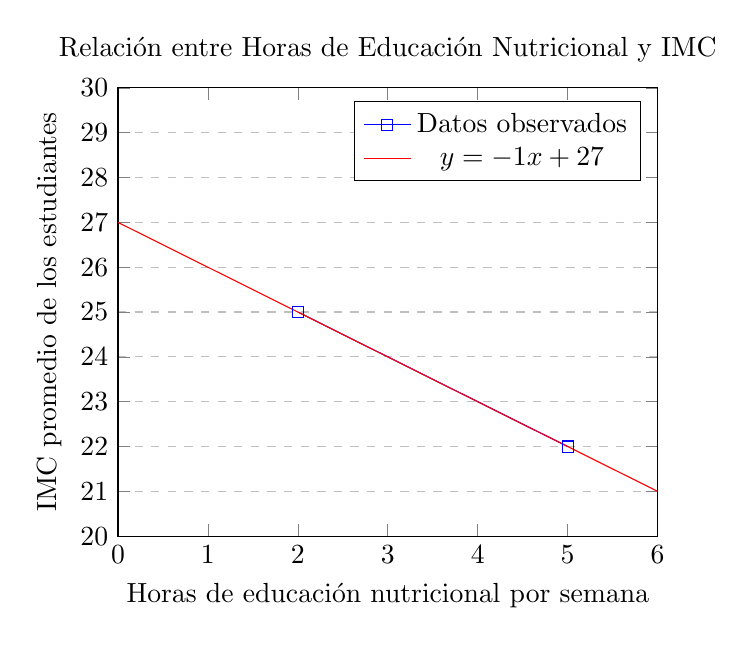
\begin{tikzpicture}
\begin{axis}[
    title={Relación entre Horas de Educación Nutricional y IMC},
    xlabel={Horas de educación nutricional por semana},
    ylabel={IMC promedio de los estudiantes},
    xmin=0, xmax=6,
    ymin=20, ymax=30,
    xtick={0,1,2,3,4,5,6},
    ytick={20,21,22,23,24,25,26,27,28,29,30},
    legend pos=north east,
    ymajorgrids=true,
    grid style=dashed,
]

\addplot[
    color=blue,
    mark=square,
    ]
    coordinates {
    (5,22)(2,25)
    };
    \addlegendentry{Datos observados}

\addplot[
    domain=0:6,
    samples=100,
    color=red,
]
{-1*x + 27};
\addlegendentry{$y=-1x+27$}

\end{axis}
\end{tikzpicture}\end{document}